\documentclass[11pt, twocolumn]{article}
\usepackage{geometry} % see geometry.pdf on how to lay out the page. There's lots.
\geometry{a4paper} % or letter or a5paper or ... etc
% \geometry{landscape} % rotated page geometry

% See the ``Article customise'' template for come common customisations
\usepackage{graphicx}
\usepackage{subcaption}
\graphicspath{ {./images/} }
\usepackage{placeins}


\usepackage{biblatex}

\title{Assignment 1 - Supervised Learning}
\author{Sebastien Thomas}

%%% BEGIN DOCUMENT
\begin{document}
    \maketitle

    \begin{abstract}
        For this assignment I will be implementing (stealing) five supervised learning algorithms and analyze two datasets. The algorithms I am going to use are Neural Networks, Boosting, Decision Tree, K-Nearest Neighbors, and Support Vector Machines. I will then compare and contrast the performance of each algorithms against the two datasets pointing interesting findings in the process.
    \end{abstract}

    \section[Problems]{Problems}
    The first problem we are going to tackle is to predict whether someone's income exceeds \$50K/yr based on census data.
    We use the dataset from UCI, \cite{adult}.
    I thought that dataset was interesting for multiple reasons.
    First it has a lot of data to train on.
    Also with the discussion happening around the country about pay disparity, I thought it was interesting to analyze how much impact someone's demographics had on their income.

    For the second problem we are going to predict whether someone has diabetes based on their medical records.
    One insteresting aspect of this dataset was the size.
    The amount of data available is low.
    Healthcare being such a big topic, I wondered if it was possible to accurately diagnose an individual even with limited prior examples.

    \section{Datasets}

    To have a better understanding of the dataset and the subsequence results, we started by analyzing the distribution of the classes in each of the training datasets. We can see, from Fig \ref{fig:balance_curve_adult}, that the Adult dataset has approximately 3 times more positive classes than negative classes. Whereas from Fig \ref{fig:balance_diabetes}, we have about 2 time more samples without diabetes than with diabetes.

    \begin{figure}[!htbp]
        \begin{subfigure}{.24\textwidth}
            \centering
            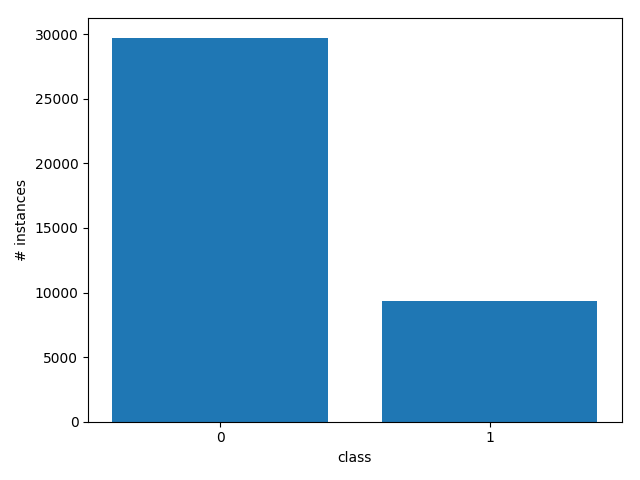
\includegraphics[width=.9\textwidth]{distribution_Adult}
            \caption{Adult}
            \label{fig:balance_curve_adult}
        \end{subfigure}
        \begin{subfigure}{.24\textwidth}
            \centering
            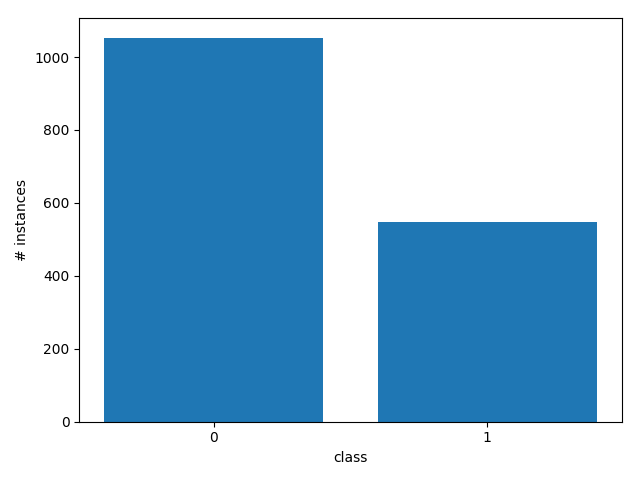
\includegraphics[width=.9\textwidth]{distribution_Diabetes}
            \caption{Diabetes}
            \label{fig:balance_diabetes}
        \end{subfigure}
        \caption{Class Distribution}
    \end{figure}
    \FloatBarrier

    The adult dataset has 48840 instances and 15 features.
    However the diabetes dataset has 2000 instances and 15 features.

    \section{Algorithms}
    \subsection{Decision Tree}

    For the decision tree algorithm, I look at the impact of the max depth and the max leaf nodes on the performance of the models. Gini index was used to split at the nodes. As we see in Fig \ref{fig:validations_Adult_DT_max_depth} we see that the model starts to overfit once the depth of the model increases past 8 for the adult dataset. However for the diabetes dataset, the overfitting seems to starts when the max depth increases past 16, Fig \ref{fig:validations_Diabetes_DT_max_depth}. One interesting observation is that the test score doesn't decrease once the model starts to overfit for the diabetes dataset, which indicate that the model is not suffering from high error due to variance. However for the adult dataset, we can see the high variance once the model starts to overfit.

    \begin{figure}[!htbp]
        \begin{subfigure}{.24\textwidth}
            \centering
            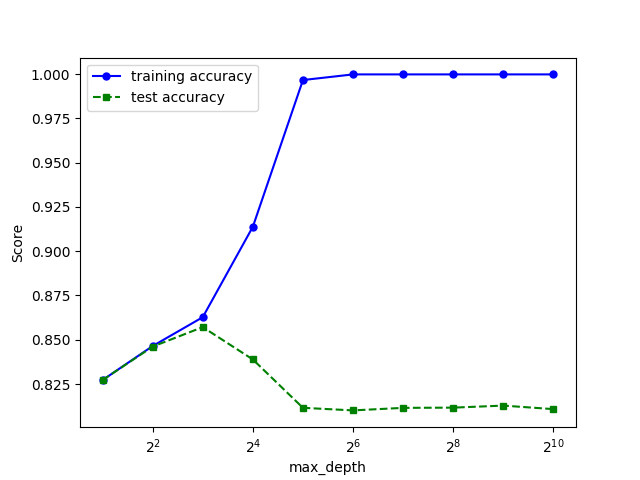
\includegraphics[width=.9\textwidth]{validations_Adult_DT_max_depth}
            \caption{Adult}
            \label{fig:validations_Adult_DT_max_depth}
        \end{subfigure}
        \begin{subfigure}{.24\textwidth}
            \centering
            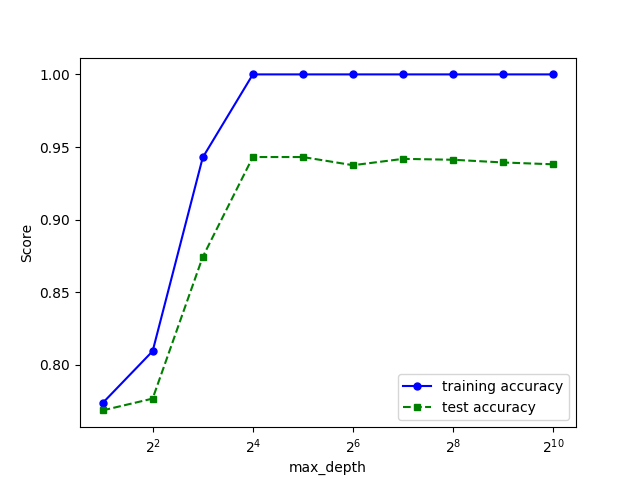
\includegraphics[width=.9\textwidth]{validations_Diabetes_DT_max_depth}
            \caption{Diabetes}
            \label{fig:validations_Diabetes_DT_max_depth}
        \end{subfigure}
        \caption{Validation Curves}
    \end{figure}
    \FloatBarrier

    For each of the datasets, we then used grid search to find the best parameters. For the adult dataset, they turned out to be: max depth = 8. And for the diabetes dataset they turned out to be: max depth = 16. We then computed the learning curves for each of the datasets. As we train on more samples for the adult dataset, we that below 10,000 samples, we have a high variance, and the curves starts converging after that, Fig \ref{fig:learnings_Adult_DT}. However, the converge at a relatively accuracy, which indicates a high bias. In comparison, the diabetes starts with a high degree of variance, and keeps improving as we add more training data, Fig \ref{fig:learnings_Diabetes_DT}. After exhausting all the training data, we see that the curves don't converge. The upwards trend of the validation curve indicates that adding more data would have likely kept increasing the accuracy of the model.

    \begin{figure}[!htbp]
        \begin{subfigure}{.24\textwidth}
            \centering
            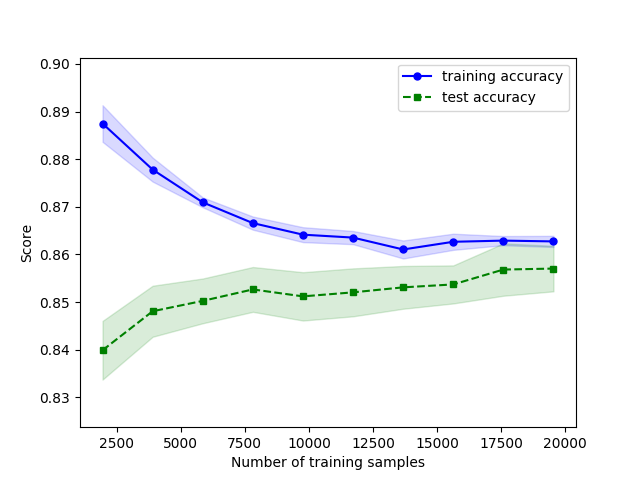
\includegraphics[width=.9\textwidth]{learnings_Adult_DT_optimized}
            \caption{Adult}
            \label{fig:learnings_Adult_DT}
        \end{subfigure}
        \begin{subfigure}{.24\textwidth}
            \centering
            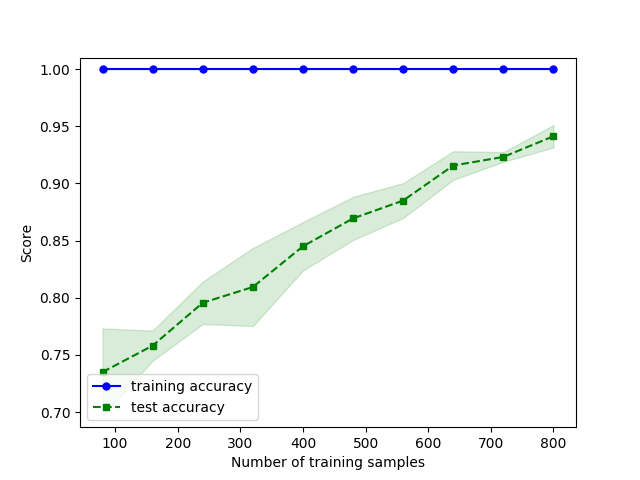
\includegraphics[width=.9\textwidth]{learnings_Diabetes_DT_optimized}
            \caption{Diabetes}
            \label{fig:learnings_Diabetes_DT}
        \end{subfigure}
        \caption{Learning Curves}
    \end{figure}
    \FloatBarrier

    \subsection{Boosting}

    When it comes to boosting, I used Ada Boost. The goal here was trying to improve the decision tree above. I first started by looking at what the impact of adding more iterators had on the performance.

    \begin{figure}[!htbp]
        \begin{subfigure}{.24\textwidth}
            \centering
            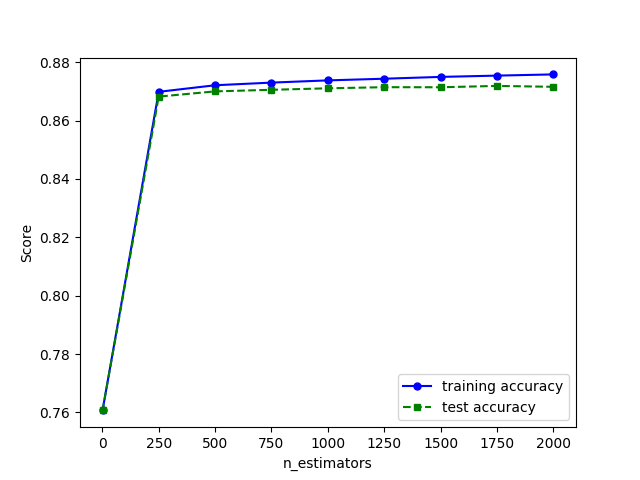
\includegraphics[width=.9\textwidth]{validations_Adult_Boosting_n_estimators}
            \caption{Adult}
            \label{fig:validations_Adult_Boosting}
        \end{subfigure}
        \begin{subfigure}{.24\textwidth}
            \centering
            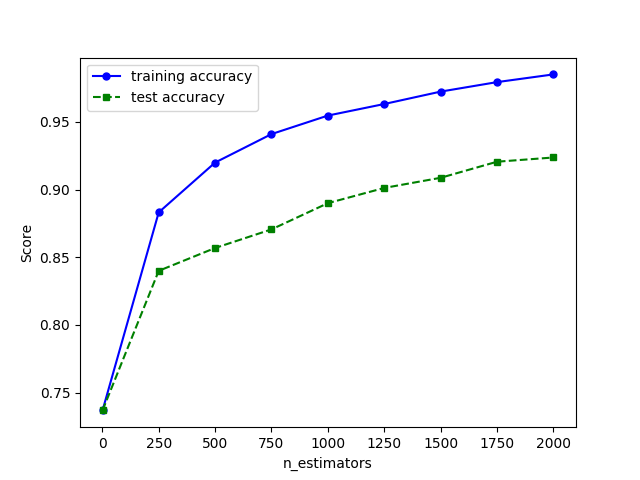
\includegraphics[width=.9\textwidth]{validations_Diabetes_Boosting_n_estimators}
            \caption{Diabetes}
            \label{fig:validations_Diabetes_Boosting}
        \end{subfigure}
        \caption{Validation Curves}
    \end{figure}
    \FloatBarrier

    We can observe that for the adult dataset, Fig \ref{fig:validations_Adult_Boosting}, the model tends to underfit between 1 to 250 iterators. After that, not only the test and training curves converge, but the test accuracy doesn't decrease. The accuracy is still low, around 0.87, which indicates a high level of bias and low variance. Adding more training sample doesn't seem like it would have made a difference as the curves stayed pretty much flat as we added more data. However for the diabetes dataset, Fig \ref{fig:validations_Diabetes_Boosting} we see a high level of variance shown by the gab between the training and the testing accuracy. Both curves also have an upwards trends, which indicates an underfitting issue. Having more training data would have likely improved the accuracy of the model.

    Again, we used grid search to find the best parameters. For each of the datasets and computed the learning curves.

    \begin{figure}[!htbp]
        \begin{subfigure}{.24\textwidth}
            \centering
            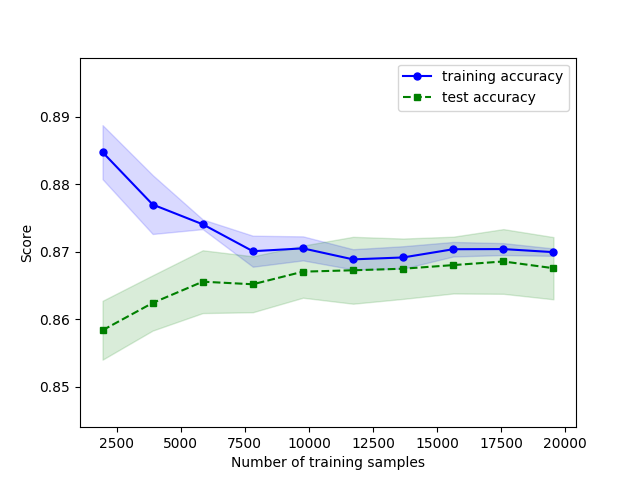
\includegraphics[width=.9\textwidth]{learnings_Adult_Boosting_optimized}
            \caption{Adult}
            \label{fig:learnings_Adult_Boosting}
        \end{subfigure}
        \begin{subfigure}{.24\textwidth}
            \centering
            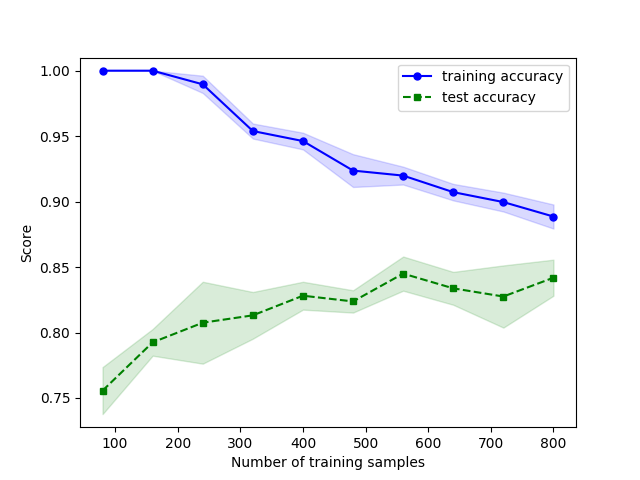
\includegraphics[width=.9\textwidth]{learnings_Diabetes_Boosting_optimized}
            \caption{Diabetes}
            \label{fig:learnings_Diabetes_Boosting}
        \end{subfigure}
        \caption{Learning Curves}
        \label{fig:learning_curves}
    \end{figure}
    \FloatBarrier

    The behavior was similar to the Decision Tree algorithm we saw earlier as Decision Tree was used as the base algorithm. For the adult dataset, Fig \ref{fig:learnings_Adult_Boosting}, the model seems to overfit somewhere between 10000 and 12500 sample size. The accuracy was still low which indicated a high level of bias. When it comes to the diabetes dataset, Fig \ref{fig:learnings_Diabetes_Boosting}, we see that the variance reduced faster, but the curves still didn't converged completely. This shows that there is still some variance and adding more training data would have likely improved the model accuracy.


    \subsection{KNN}

    For the KNN algorithm, I looked at the impact of adding additional neighbors had on the performance of the model for each of the datasets. For the adult dataset, Fig \ref{fig:validations_Adult_KNN}, we see a high level of bias as the curves converged at a low accuracy. But we see that if we added more neighbors, the model would have probably generalized more, and reduce the variance. On the other hand for the diabetes dataset, Fig \ref{fig:validations_Diabetes_KNN}, as we added more and more neighbors, both test accuracy and training accuracy continued to decrease. Which indicated a high level of bias. In both cases however, we see a high variance with less than 15 neighbors.

    \begin{figure}[!htbp]
        \begin{subfigure}{.24\textwidth}
            \centering
            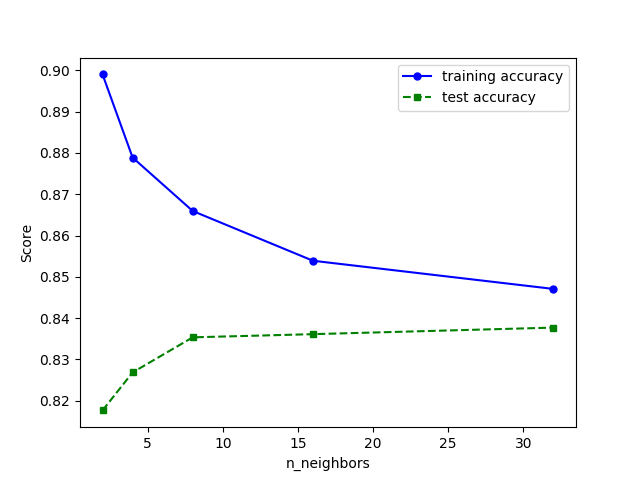
\includegraphics[width=.9\textwidth]{validations_Adult_KNN_n_neighbors}
            \caption{Adult}
            \label{fig:validations_Adult_KNN}
        \end{subfigure}
        \begin{subfigure}{.24\textwidth}
            \centering
            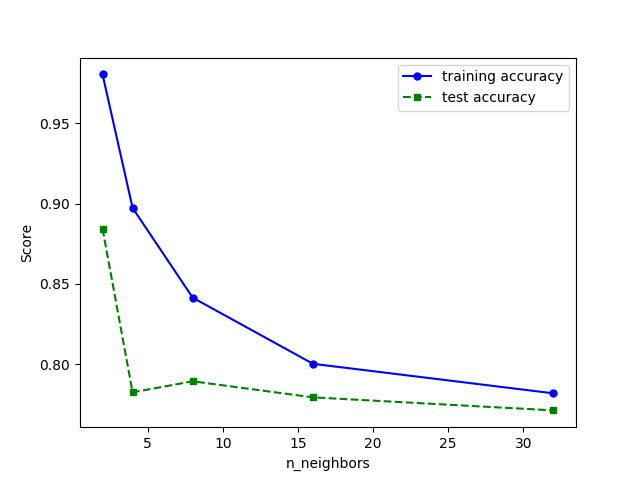
\includegraphics[width=.9\textwidth]{validations_Diabetes_KNN_n_neighbors}
            \caption{Diabetes}
            \label{fig:validations_Diabetes_KNN}
        \end{subfigure}
        \caption{Validation Curves}
    \end{figure}
    \FloatBarrier

    After using grid search to find the best parameters, which turned out to be 32 neighbors for the adult dataset, and 2 neighbors for the diabetes dataset, we computed the learning curves to understand how much we benefit from adding more training samples.

    \begin{figure}[!htbp]
        \begin{subfigure}{.24\textwidth}
            \centering
            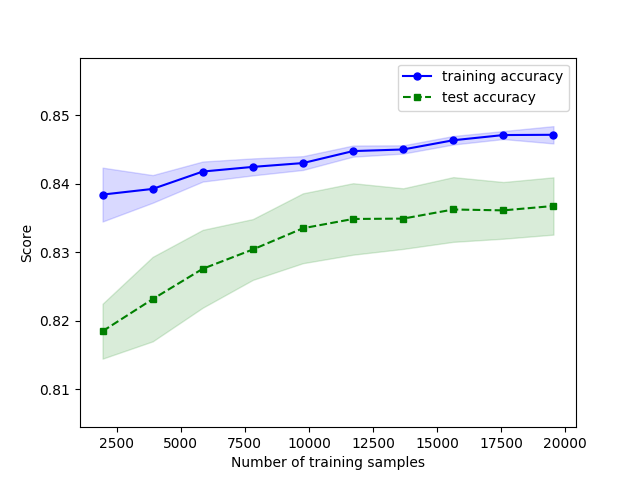
\includegraphics[width=.9\textwidth]{learnings_Adult_KNN_optimized}
            \caption{Adult}
            \label{fig:learnings_Adult_KNN}
        \end{subfigure}
        \begin{subfigure}{.24\textwidth}
            \centering
            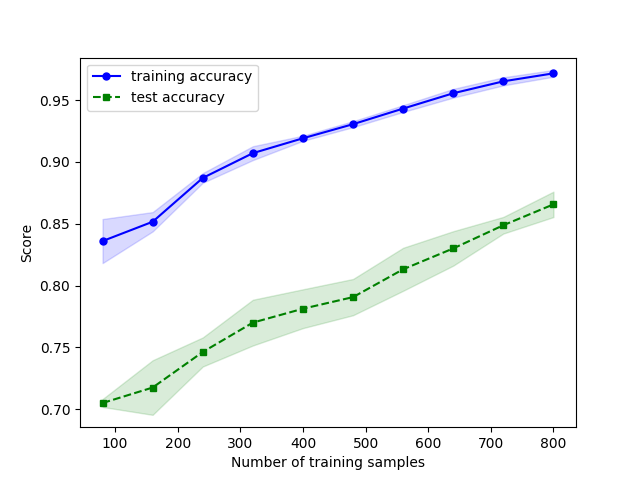
\includegraphics[width=.9\textwidth]{learnings_Diabetes_KNN_optimized}
            \caption{Diabetes}
            \label{fig:learnings_Diabetes_KNN}
        \end{subfigure}
        \caption{Learning Curves}
    \end{figure}
    \FloatBarrier

    An interesting observation is that in both cases, both the training and the test accuracy kept increasing as we added more training samples. The adult dataset, Fig \ref{fig:learnings_Adult_KNN} exhibited less variance that the diabetes dataset, Fig \ref{fig:learnings_Diabetes_KNN}. The upwards trajectory of both curves indicates that adding more training data would have increased the accuracy, and decrease the level of undefitting that we are seeing.

    \subsection{SVC Linear}

    For the SVC algorithm, we first looked at the linear kernel. The expectation was that if the datasets were linearly separable, this algorithm would perform well. We looked at the impact of the regularization parameter, C, on the performance of the model. For the adult dataset, Fig \ref{fig:validations_Adult_SVC_Linear_C}, we saw that both training and testing validation curves converged at all time, which was a sign of low variance. We see the accuracy decrease drastically once C increased passed 10. We observed pretty much the same for the diabetes dataset, Fig \ref{fig:validations_Diabetes_SVC_Linear_C}.

    \begin{figure}[!htbp]
        \begin{subfigure}{.24\textwidth}
            \centering
            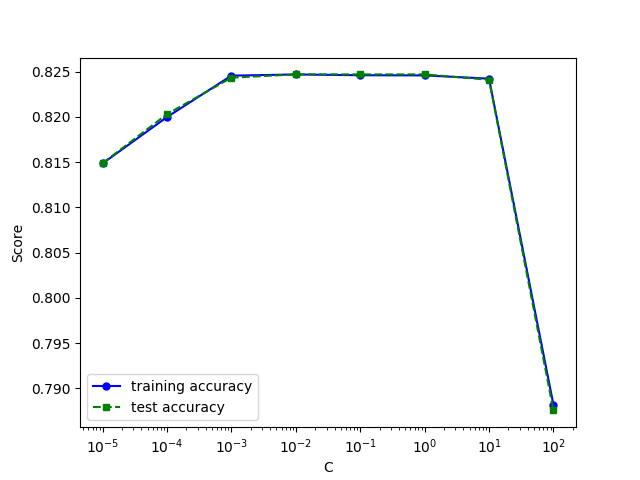
\includegraphics[width=.9\textwidth]{validations_Adult_SVC_Linear_C}
            \caption{Adult}
            \label{fig:validations_Adult_SVC_Linear_C}
        \end{subfigure}
        \begin{subfigure}{.24\textwidth}
            \centering
            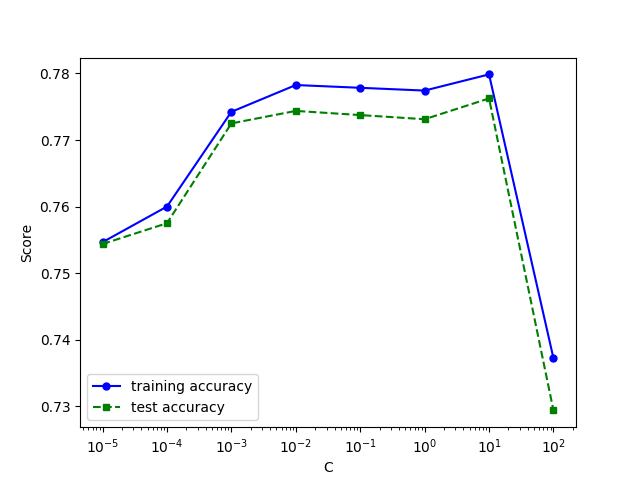
\includegraphics[width=.9\textwidth]{validations_Diabetes_SVC_Linear_C}
            \caption{Diabetes}
            \label{fig:validations_Diabetes_SVC_Linear_C}
        \end{subfigure}
        \caption{Validation Curves}
    \end{figure}
    \FloatBarrier

    After using grid search which confirmed the the value for C, we computed the learning curves for each datasets.

    \begin{figure}[!htbp]
        \begin{subfigure}{.24\textwidth}
            \centering
            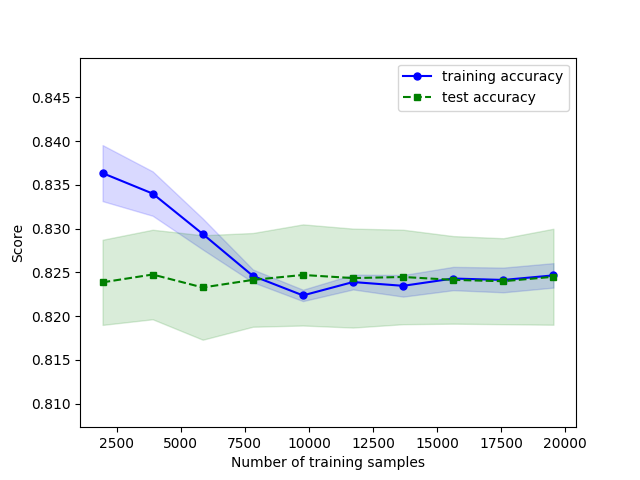
\includegraphics[width=.9\textwidth]{learnings_Adult_SVC_Linear_optimized}
            \caption{Adult}
            \label{fig:learnings_Adult_SVC_Linear_optimized}
        \end{subfigure}
        \begin{subfigure}{.24\textwidth}
            \centering
            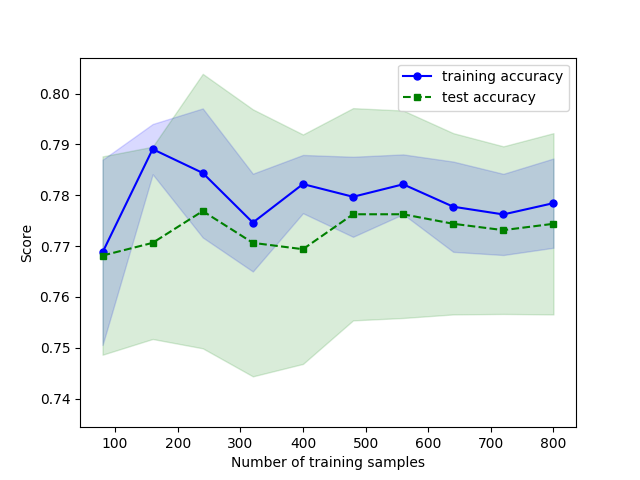
\includegraphics[width=.9\textwidth]{learnings_Diabetes_SVC_Linear_optimized}
            \caption{Diabetes}
            \label{fig:learnings_Diabetes_SVC_Linear_optimized}
        \end{subfigure}
        \caption{Learning Curves}
    \end{figure}
    \FloatBarrier

    We see that the training and test curves converged early for the adult dataset, Fig \ref{fig:learnings_Adult_SVC_Linear_optimized}. The accuracy was low, which indicated high bias. For the diabetes dataset. Fig \ref{fig:learnings_Diabetes_SVC_Linear_optimized}, the curved never completely converged, which shows some variance, and the accuracy was also low, which indicates high bias. The low accuracy can also be attributed to the fact that none of the datasets were linearly separable.

    \subsection{SVC RBF}

    Next we looked at the SVC algorithm again, but using the Gaussian RBF(Radial Basis Function) kernel as it seemed that the data was not linearly separable. For the adult dataset, Fig \ref{fig:validations_Adult_SVC_RBF_C}, again we saw that the model started to overfit when the value of C increased pass 10. After this we started seeing a high variance. On the other hand for the diabetes dataset, Fig \ref{fig:validations_Diabetes_SVC_RBF_C}, We never really saw overfiting happened. Both the training and testing curves kept improving as we increased the value of C. This happens because the diabetes dataset, even though small, contains a very representative sample of the reality, including extreme examples.

    \begin{figure}[!htbp]
        \begin{subfigure}{.24\textwidth}
            \centering
            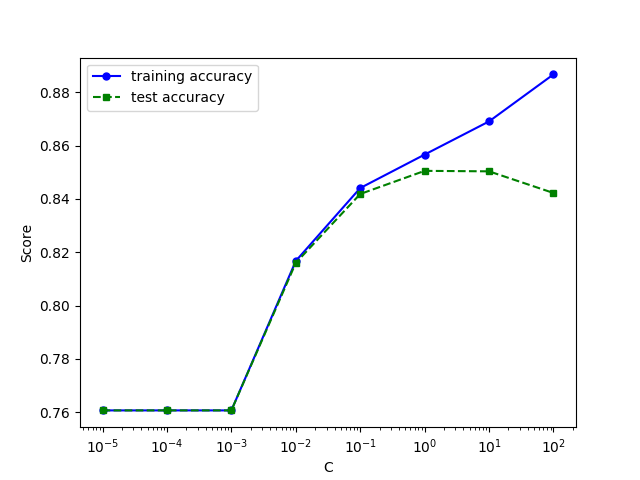
\includegraphics[width=.9\textwidth]{validations_Adult_SVC_RBF_C}
            \caption{Adult}
            \label{fig:validations_Adult_SVC_RBF_C}
        \end{subfigure}
        \begin{subfigure}{.24\textwidth}
            \centering
            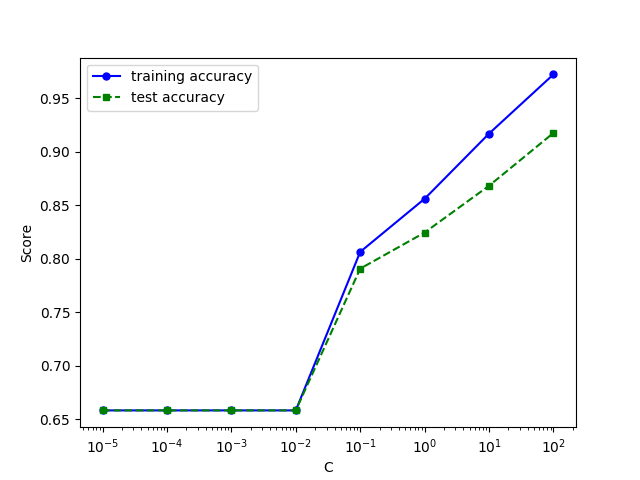
\includegraphics[width=.9\textwidth]{validations_Diabetes_SVC_RBF_C}
            \caption{Diabetes}
            \label{fig:validations_Diabetes_SVC_RBF_C}
        \end{subfigure}
        \caption{Validation Curves}
    \end{figure}
    \FloatBarrier

    After again using grid search to find the best parameters, we computed the learning curves for each of the datasets.

    \begin{figure}[!htbp]
        \begin{subfigure}{.24\textwidth}
            \centering
            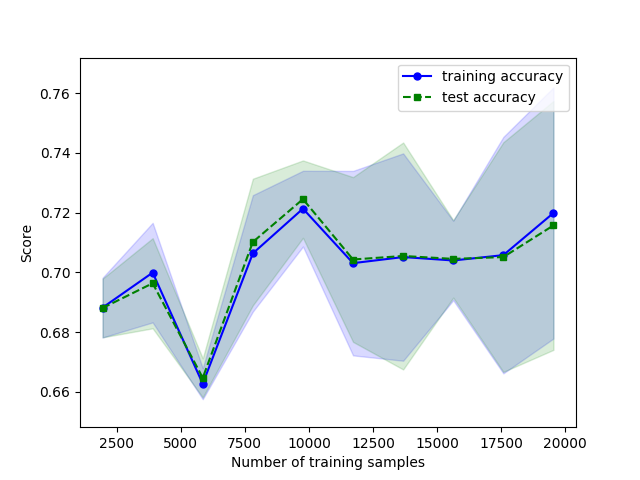
\includegraphics[width=.9\textwidth]{learnings_Adult_SVC_RBF_optimized}
            \caption{Adult}
            \label{fig:learnings_Adult_SVC_RBF_optimized}
        \end{subfigure}
        \begin{subfigure}{.24\textwidth}
            \centering
            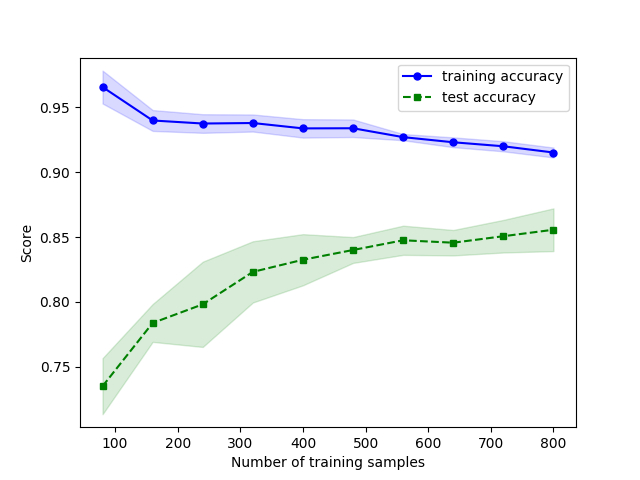
\includegraphics[width=.9\textwidth]{learnings_Diabetes_SVC_RBF_optimized}
            \caption{Diabetes}
            \label{fig:learnings_Diabetes_SVC_RBF_optimized}
        \end{subfigure}
        \caption{Learning Curves}
    \end{figure}
    \FloatBarrier

    As we saw for the adult dataset, Fig \ref{fig:learnings_Adult_SVC_RBF_optimized}, the curves converged at a very low accuracy, which indicates a high level of bias. I am not sure if adding more training samples would have improved the accuracy. However, for the diabetes dataset, Fig \ref{fig:learnings_Diabetes_SVC_RBF_optimized}, we see that the model kept improving as we added more training data. The accuracy was higher than all the models we've seen so far, this shows the power of the rbf kernel which is able to model very complex problems. We still saw a high variance, which could have been improved if we had more training data.

    \subsection{MLP}

    Finally the last algorithm we looked at is the Multilayer Perceptron, MLP. For both we looked at the effect of increasing the number of nodes in a 1 layer network. For the adult dataset, Fig \ref{fig:validations_Adult_MLP_hidden_layer_sizes_1_layer}, we see that the model starts to overfit once we added more that 16 nodes in the layer. Pass that point, we see a large degree of variance. On the other hand for the diabetes dataset, Fig \ref{fig:validations_Diabetes_MLP_hidden_layer_sizes_1_layer}, we see that overfiting happens around 64 nodes in the layer. For both we kept the max iterations at 200.

    \begin{figure}[!htbp]
        \begin{subfigure}{.24\textwidth}
            \centering
            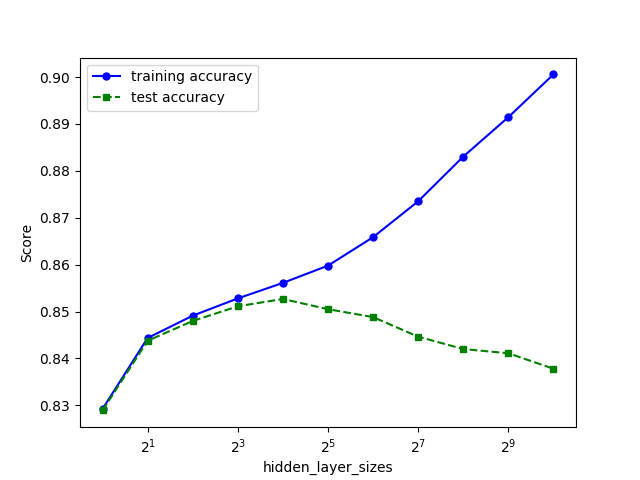
\includegraphics[width=.9\textwidth]{validations_Adult_MLP_hidden_layer_sizes_1_layer}
            \caption{Adult}
            \label{fig:validations_Adult_MLP_hidden_layer_sizes_1_layer}
        \end{subfigure}
        \begin{subfigure}{.24\textwidth}
            \centering
            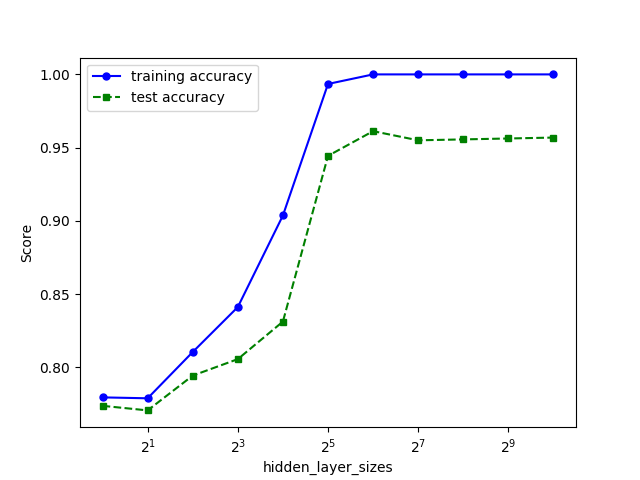
\includegraphics[width=.9\textwidth]{validations_Diabetes_MLP_hidden_layer_sizes_1_layer}
            \caption{Diabetes}
            \label{fig:validations_Diabetes_MLP_hidden_layer_sizes_1_layer}
        \end{subfigure}
        \caption{Validation Curves}
    \end{figure}
    \FloatBarrier

    After computing the learning curves with the best parameters found using grid search we had some interesting observations.

    \begin{figure}[!htbp]
        \begin{subfigure}{.24\textwidth}
            \centering
            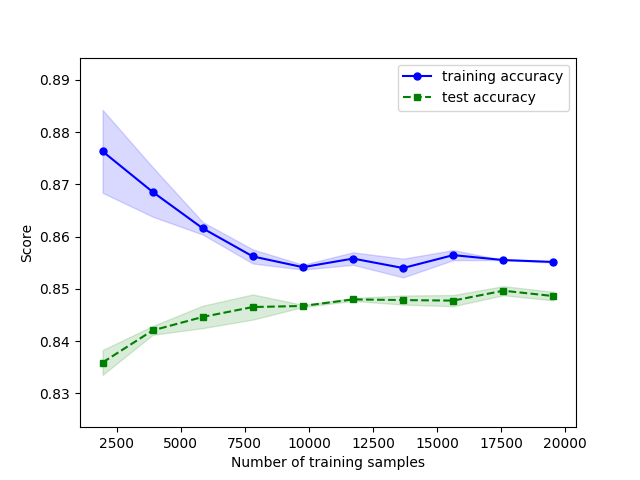
\includegraphics[width=.9\textwidth]{learnings_Adult_MLP_optimized}
            \caption{Adult}
            \label{fig:learnings_Adult_MLP_optimized}
        \end{subfigure}
        \begin{subfigure}{.24\textwidth}
            \centering
            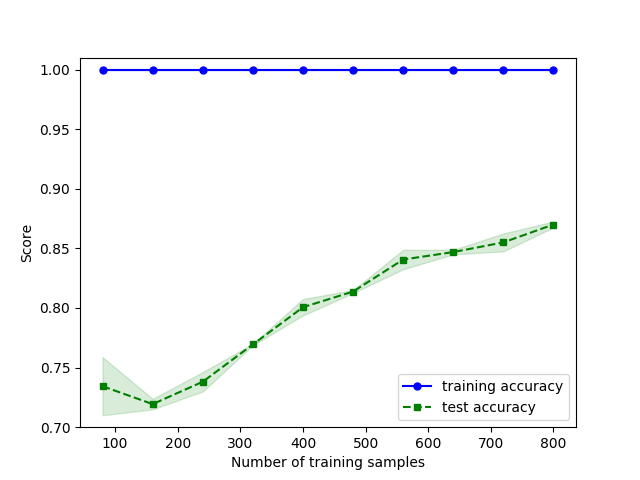
\includegraphics[width=.9\textwidth]{learnings_Diabetes_MLP_optimized}
            \caption{Diabetes}
            \label{fig:learnings_Diabetes_MLP_optimized}
        \end{subfigure}
        \caption{Learning Curves}
    \end{figure}
    \FloatBarrier

    For the adult dataset, Fig \ref{fig:learnings_Adult_MLP_optimized}, we see that for less than 10000 training samples, we have high variance. Then as we added more data, the accuracy improved slightly but we still saw some variance. Adding more sample may or may not have improved the accuracy even more. However, for the diabetes dataset, Fig \ref{fig:learnings_Diabetes_MLP_optimized}, we had very high variance and adding more training data would have likely improved the accuracy of the model.

    \section{Comparisons}

    As we started comparing the different algorithms, the first metrics we looked at was the scalability of the model. How long it takes for the model to train as we add more training data? We saw that for the diabetes dataset, Fig \ref{fig:scalability_Diabetes_optimized}, it appears that all the models had constant training time. This is only because we only trained on a small sample of data. Even then, we saw that the neural network still grew exponentially as we added more data. The adult dataset, Fig \ref{fig:scalability_Adult_optimized}, which had way more training data, showed a better picture of the scalability of the algorithms. We see that as we added more data, the training time for the SVC with linear kernel grew the fastest. This is likely due to the fact that this dataset is not linearly separable.

    \begin{figure}[!htbp]
        \begin{subfigure}{.24\textwidth}
            \centering
            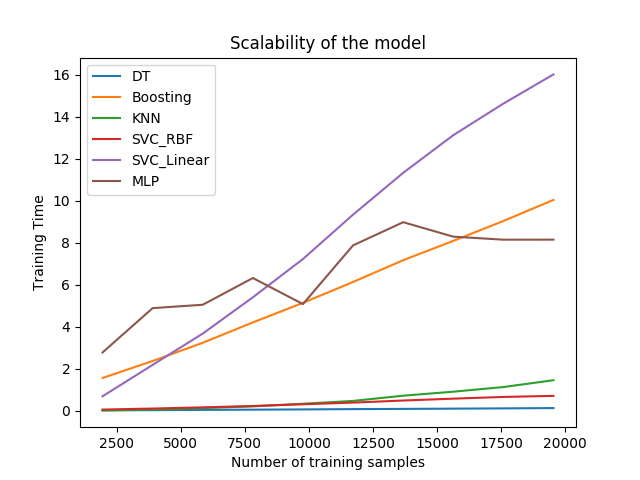
\includegraphics[width=.9\textwidth]{scalability_Adult_optimized}
            \caption{Adult}
            \label{fig:scalability_Adult_optimized}
        \end{subfigure}
        \begin{subfigure}{.24\textwidth}
            \centering
            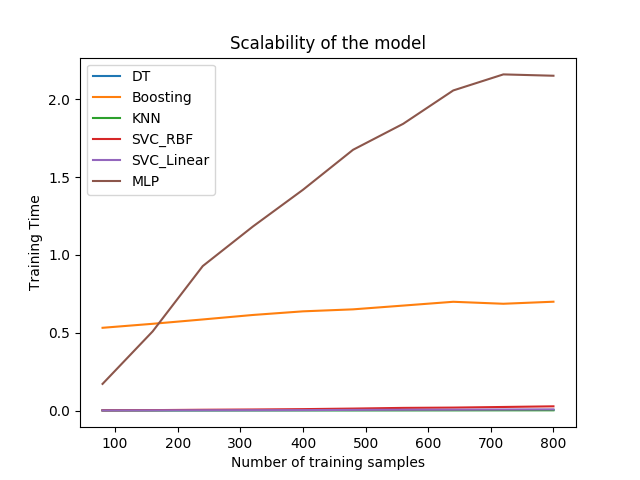
\includegraphics[width=.9\textwidth]{scalability_Diabetes_optimized}
            \caption{Diabetes}
            \label{fig:scalability_Diabetes_optimized}
        \end{subfigure}
        \caption{Model Scalability}
    \end{figure}
    \FloatBarrier

    As far as the relation between the training time and the accuracy of the model, the only conclusive observation we had was the fact that for the diabetes dataset, Fig \ref{fig:performance_Diabetes_optimized}, the longer we training the neural network, the better performance we achieved. For the other algorithms we didn't see any significant improvements as we trained the models longer. This is likely due to either the lack of training data in the case of the diabetes dataset, or the problem itself not being represented well using those supervised techniques.

    \begin{figure}[!htbp]
        \begin{subfigure}{.24\textwidth}
            \centering
            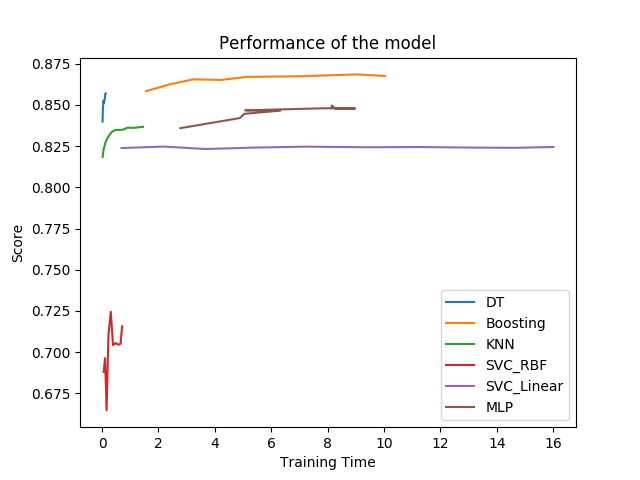
\includegraphics[width=.9\textwidth]{performance_Adult_optimized}
            \caption{Adult}
            \label{fig:performance_Adult_optimized}
        \end{subfigure}
        \begin{subfigure}{.24\textwidth}
            \centering
            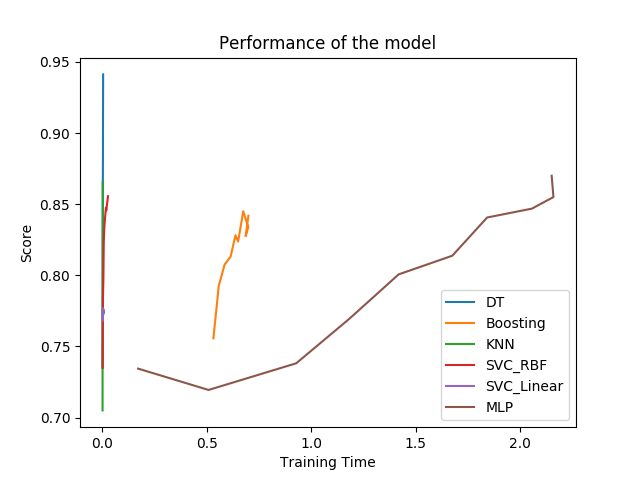
\includegraphics[width=.9\textwidth]{performance_Diabetes_optimized}
            \caption{Diabetes}
            \label{fig:performance_Diabetes_optimized}
        \end{subfigure}
        \caption{Time vs Score}
    \end{figure}
    \FloatBarrier

    \section{Conclusion}

    Overall it was a great experiment. We got to see how different algorithms performs depending on the type of problem chosen. Overall we see Decision tree perform better for both dataset, as it had a better accuracy. In the case of the adult dataset, Fig \ref{fig:comparisons_Adult}, using boosting slightly improved the overall score of the decision tree algorithm. This is due to the nature of boosting to reduce overfitting and generalize the models better by reducing the impact of outliers. The worst performing algorithm for the adult dataset was the SVM with rbf kernel. This was likely due to the fact that this model was too complex for the chosen problem. When it comes to the diabetes dataset, Fig \ref{fig:comparisons_Diabetes}, the accuracy scores were not drastically different, however we saw the SVM with rbf kernel perform quite well, compared to the linear kernel. This highlights the power of the rbf kernel to elevate the data to high dimensions in order to separate the data. The biggest issue we saw with the diabetes dataset was the lack of training data. Throughout the experiment we used cross-validation to try to reduce overfitting.

    \begin{figure}[!htbp]
        \begin{subfigure}{.24\textwidth}
            \centering
            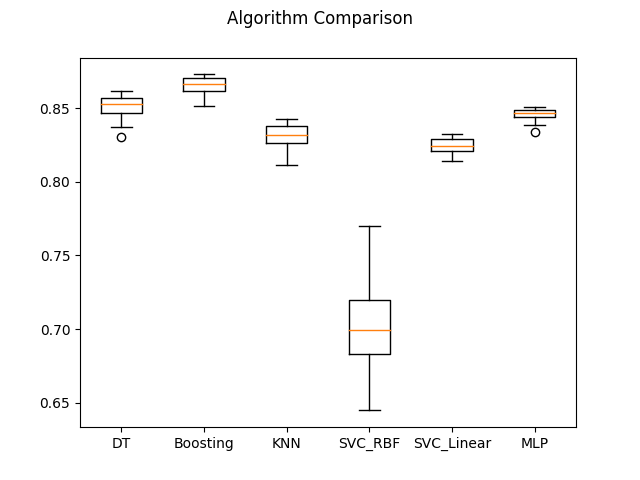
\includegraphics[width=.9\textwidth]{Adult_optimized}
            \caption{Adult}
            \label{fig:comparisons_Adult}
        \end{subfigure}
        \begin{subfigure}{.24\textwidth}
            \centering
            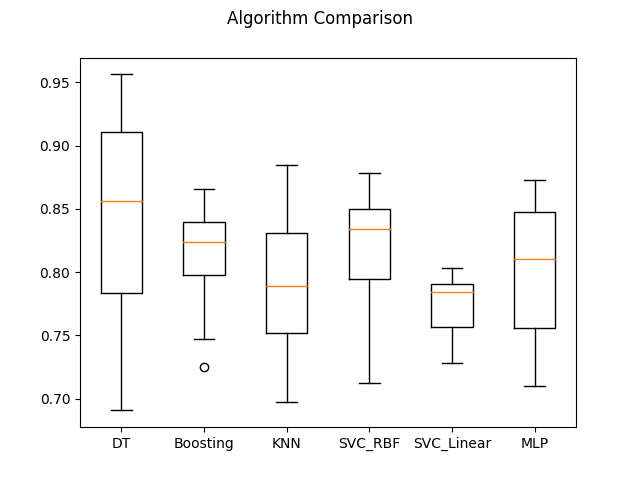
\includegraphics[width=.9\textwidth]{Diabetes_optimized}
            \caption{Diabetes}
            \label{fig:comparisons_Diabetes}
        \end{subfigure}
        \caption{Performance}
    \end{figure}
    \FloatBarrier

    \newpage
    \begin{thebibliography}{9}
        \bibitem{adult}
        Ronny Kohavi and Barry Becker
        Data Mining and Visualization
        Silicon Graphics.
        \\\texttt{https://archive.ics.uci.edu/ml/datasets/Census+Income}

        \bibitem{diabetes}
        Michael Kahn, MD, PhD, Washington University, St. Louis, MO
        \\\texttt{https://archive.ics.uci.edu/ml/datasets/diabetes}

    \end{thebibliography}

\end{document}